%%%%%%%%%%%%%%%%%%%%%%%%%%%%%%%%%%%%%%%%%%%%%%%%%%%%%%%%%%%%%%%%%%%%%%%%%%%%%%%%%%
\begin{frame}[fragile]\frametitle{}

\begin{center}
{\Large BERT embeddings}

\end{center}
\end{frame}

%%%%%%%%%%%%%%%%%%%%%%%%%%%%%%%%%%%%%%%%%%%%%%%%%%%%%%%%%%%%%%%%%%%%%%%%%%%%%%%%%%
\begin{frame}[fragile]\frametitle{}

\begin{center}
{\Large Introduction to BERT}

{\tiny (Sentiment Analysis with BERT and Transformers by Hugging Face using PyTorch and Python - Curiousily  

Demystifying BERT: A Comprehensive Guide to the Groundbreaking NLP Framework - 
MOHD SANAD ZAKI RIZVI)}

\end{center}
\end{frame}

%%%%%%%%%%%%%%%%%%%%%%%%%%%%%%%%%%%%%%%%%%%%%%%%%%%%%%%%%%%%%%%%%%%%%%%%%%%%%%%%%%
\begin{frame}[fragile]\frametitle{What is BERT?}
BERT stands for Bidirectional Encoder Representations from Transformers.

\begin{itemize}
\item Bidirectional: Look back (at the previous words) and forward (at the next words)
\item Transformers: Reads entire sequences of tokens at once. In a sense, the model is non-directional, while LSTMs read sequentially (left-to-right or right-to-left). The attention mechanism allows for learning contextual relations between words.
\end{itemize}
\end{frame}

%%%%%%%%%%%%%%%%%%%%%%%%%%%%%%%%%%%%%%%%%%%%%%%%%%%%%%%%%%%%%%%%%%%%%%%%%%%%%%%%%%
\begin{frame}[fragile]\frametitle{Goal of BERT}

\begin{itemize}
\item BERT was trained by masking 15\% of the tokens with the goal to guess them. \lstinline|That's [mask] she [mask] -> That's what she said|
\item Given a pair of two sentences, the task is to say whether or not the second follows the first (binary classification).
\begin{lstlisting}
Input = [CLS] That's [mask] she [mask]. [SEP] Hahaha, nice! [SEP]

Label = IsNext

Input = [CLS] That's [mask] she [mask]. [SEP] Dwight, you ignorant [mask]! [SEP]

Label = NotNext
\end{lstlisting}

\end{itemize}
\end{frame}

%%%%%%%%%%%%%%%%%%%%%%%%%%%%%%%%%%%%%%%%%%%%%%%%%%%%%%%%%%%%%%%%%%%%%%%%%%%%%%%%%%
\begin{frame}[fragile]\frametitle{Training of BERT}
The training corpus was comprised of

\begin{itemize}
\item  Toronto Book Corpus (800M words)
\item English Wikipedia (2,500M words). 
\end{itemize}

While the original Transformer has an encoder (for reading the input) and a decoder (that makes the prediction), BERT uses only the decoder.

\end{frame}

%%%%%%%%%%%%%%%%%%%%%%%%%%%%%%%%%%%%%%%%%%%%%%%%%%%%%%%%%%%%%%%%%%%%%%%%%%%%%%%%%%
\begin{frame}[fragile]\frametitle{Architecture of BERT}

\begin{itemize}
\item  BERT is simply a pre-trained stack of Transformer Encoders. How many Encoders? 
\item BERT Base: 12 layers (transformer blocks), 12 attention heads, and 110 million parameters
\item BERT Large: 24 layers (transformer blocks), 16 attention heads and, 340 million parameters

\end{itemize}

% \begin{center}
% 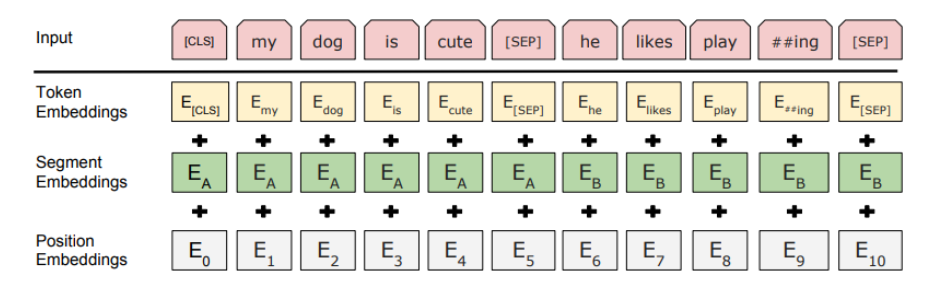
\includegraphics[width=0.3\linewidth,keepaspectratio]{bert1}
% \end{center}

% {\tiny (Ref: The Illustrated BERT, ELMo, and co. (How NLP Cracked Transfer Learning) - Jay Alammar )}

\end{frame}

%%%%%%%%%%%%%%%%%%%%%%%%%%%%%%%%%%%%%%%%%%%%%%%%%%%%%%%%%%%%%%%%%%%%%%%%%%%%%%%%%%
\begin{frame}[fragile]\frametitle{Using BERT}
The training corpus was comprised of

\begin{itemize}

\item You can do Transfer Learning (thanks to the ideas from OpenAI Transformer) with BERT for many NLP tasks - Classification, Question Answering, Entity Recognition, etc. 

\item You can train with small amounts of data and achieve great performance!
\end{itemize}

\end{frame}

%%%%%%%%%%%%%%%%%%%%%%%%%%%%%%%%%%%%%%%%%%%%%%%%%%%%%%%%%%%%%%%%%%%%%%%%%%%%%%%%%%
\begin{frame}[fragile]\frametitle{Text Preprocessing in BERT}

Every input embedding is a combination of 3 embeddings:

\begin{itemize}
\item Position Embeddings: Added to overcome the limitation of Transformer which, unlike an RNN, is not able to capture ``sequence'' or ``order'' information
\item Segment Embeddings: BERT can also take sentence pairs as inputs for tasks (Question-Answering). All the tokens marked as EA belong to sentence A (and similarly for EB)
\item Token Embeddings:  Learned for the specific token from the WordPiece token vocabulary
\end{itemize}

For a given token, its input representation is constructed by summing the corresponding token, segment, and position embeddings.

\begin{center}
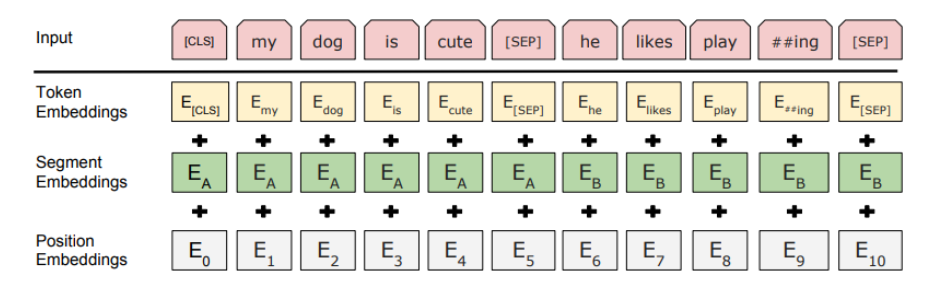
\includegraphics[width=0.8\linewidth,keepaspectratio]{bert1}
\end{center}

\end{frame}

%%%%%%%%%%%%%%%%%%%%%%%%%%%%%%%%%%%%%%%%%%%%%%%%%%%%%%%%%%%%%%%%%%%%%%%%%%%%%%%%%%
\begin{frame}[fragile]\frametitle{}

\begin{center}
{\Large Using BERT}

{\tiny (Understanding BERT — Word Embeddings - Dharti Dhami)}

\end{center}
\end{frame}



%%%%%%%%%%%%%%%%%%%%%%%%%%%%%%%%%%%%%%%%%%%%%%%%%%%%%%%%%%%%%%%%%%%%%%%%%%%%%%%%%%
\begin{frame}[fragile]\frametitle{How to use BERT}
\begin{itemize}
\item Input: Text filled between tokens ``[CLS]'' at start and ``[SEP]'' as separattors for each text blob. 
\item CLS represents classification tasks. 
\item Both tokens are a must, even if there is just one sentence, or we are not using BERT for Classification.
\item This is how BERT has been pre-trained. So, need to match that.
\item One sentence as input: \lstinline|[CLS] The man went to the store. [SEP]|
\item Two sentences as input: \lstinline|[CLS] The man went to the store. [SEP] He bought a gallon of milk.|
\end{itemize}
\end{frame}

%%%%%%%%%%%%%%%%%%%%%%%%%%%%%%%%%%%%%%%%%%%%%%%%%%%%%%%%%%%%%%%%%%%%%%%%%%%%%%%%%%
\begin{frame}[fragile]\frametitle{Steps for Word Vectors}
\begin{itemize}
\item Add special tokens to text
\item Tokenize the updated text.
\end{itemize}
\begin{lstlisting}
text = "Here is the sentence I want embeddings for."
marked_text = "[CLS] " + text + " [SEP]"

# Tokenize our sentence with the BERT tokenizer.
tokenized_text = tokenizer.tokenize(marked_text)

# Print out the tokens.
print (tokenized_text)

['[CLS]', 'here', 'is', 'the', 'sentence', 'i', 'want', 'em', '##bed', '##ding', '##s', 'for', '.', '[SEP]']
\end{lstlisting}

Seeing some broken tokens?
\end{frame}

%%%%%%%%%%%%%%%%%%%%%%%%%%%%%%%%%%%%%%%%%%%%%%%%%%%%%%%%%%%%%%%%%%%%%%%%%%%%%%%%%%
\begin{frame}[fragile]\frametitle{Broken Tokens}
\begin{itemize}
\item the word ``embeddings'' is represented: \lstinline|['em', '##bed', '##ding', '##s']|
\item The original word has been split into smaller subwords and characters.
\item Reason: BERT vocabulary is of just 30k words.
\item So, ALL words in the world can not have a vector.
\item For out-of-vocab words, they are split and seen if the sub-words are present in vocab.
\item As a last resort decompose the word into individual characters
\item With this, any word can be represented, at the very least, by characters.
\end{itemize}

\end{frame}


%%%%%%%%%%%%%%%%%%%%%%%%%%%%%%%%%%%%%%%%%%%%%%%%%%%%%%%%%%%%%%%%%%%%%%%%%%%%%%%%%%
\begin{frame}[fragile]\frametitle{Tokens to IDs}
\begin{itemize}
\item Tokenizer converts sentence into tokens
\item Tokens are indexed and their id map is populated.
\item Example: ``After stealing money from the bank vault, the bank robber was seen fishing on the Mississippi river bank.''
\item Note: word ``bank'' appears twice with a different meaning.
\end{itemize}

\end{frame}

%%%%%%%%%%%%%%%%%%%%%%%%%%%%%%%%%%%%%%%%%%%%%%%%%%%%%%%%%%%%%%%%%%%%%%%%%%%%%%%%%%
\begin{frame}[fragile]\frametitle{Tokens to IDs}

\begin{lstlisting}
# Define a new example sentence with multiple meanings of the word "bank"
text = "After stealing money from the bank vault, the bank robber was seen " \
       "fishing on the Mississippi river bank."
# Add the special tokens.
marked_text = "[CLS] " + text + " [SEP]"

# Split the sentence into tokens.
tokenized_text = tokenizer.tokenize(marked_text)

# Map the token strings to their vocabulary indeces.
indexed_tokens = tokenizer.convert_tokens_to_ids(tokenized_text)

# Display the words with their indeces.
for tup in zip(tokenized_text, indexed_tokens):
    print('{:<12} {:>6,}'.format(tup[0], tup[1]))

\end{lstlisting}

\end{frame}

%%%%%%%%%%%%%%%%%%%%%%%%%%%%%%%%%%%%%%%%%%%%%%%%%%%%%%%%%%%%%%%%%%%%%%%%%%%%%%%%%%
\begin{frame}[fragile]\frametitle{Tokens to IDs}

\begin{lstlisting}
[CLS]           101
after         2,044
stealing     11,065
money         2,769
from          2,013
the           1,996
bank          2,924
vault        11,632
,             1,010
the           1,996
bank          2,924
robber       27,307
was           2,001
seen          2,464
fishing       5,645
on            2,006
the           1,996
mississippi   5,900
river         2,314
bank          2,924
.             1,012
[SEP]           102
\end{lstlisting}

\end{frame}

%%%%%%%%%%%%%%%%%%%%%%%%%%%%%%%%%%%%%%%%%%%%%%%%%%%%%%%%%%%%%%%%%%%%%%%%%%%%%%%%%%
\begin{frame}[fragile]\frametitle{Sentences to IDs}
\begin{itemize}
\item Need to distinguish sentences by their own IDs
\item For each token in ``tokenized\_text'', we must specify which sentence it belongs to: sentence 0 (a series of 0s) or sentence 1 (a series of 1s). 
\end{itemize}

\begin{lstlisting}
# Mark each of the 22 tokens as belonging to sentence "1".
segments_ids = [1] * len(tokenized_text)
print (segments_ids)

[1, 1, 1, 1, 1, 1, 1, 1, 1, 1, 1, 1, 1, 1, 1, 1, 1, 1, 1, 1, 1, 1]

tokens_tensor = torch.tensor([indexed_tokens])
segments_tensors = torch.tensor([segments_ids])
\end{lstlisting}

\end{frame}

%%%%%%%%%%%%%%%%%%%%%%%%%%%%%%%%%%%%%%%%%%%%%%%%%%%%%%%%%%%%%%%%%%%%%%%%%%%%%%%%%%
\begin{frame}[fragile]\frametitle{Extracting Embeddings}
\begin{itemize}
\item Convert our data to tensors(input format for the model)
\item Call the BERT model.
\item output\_hidden\_states = True, Whether the model returns all hidden-states.
\end{itemize}


\begin{lstlisting}
# Load pre-trained model (weights)
model = BertModel.from_pretrained('bert-base-uncased',
                                  output_hidden_states = True, 
                                  )
# Put the model in "evaluation" mode, meaning feed-forward operation.
model.eval()
\end{lstlisting}

\end{frame}

%%%%%%%%%%%%%%%%%%%%%%%%%%%%%%%%%%%%%%%%%%%%%%%%%%%%%%%%%%%%%%%%%%%%%%%%%%%%%%%%%%
\begin{frame}[fragile]\frametitle{Evaluate Embeddings}
\begin{itemize}
\item Evaluate BERT on example text
\item Fetch the hidden states of the network!
\end{itemize}


\begin{lstlisting}
# Run the text through BERT, and collect all of the hidden states produced
# from all 12 layers. 

with torch.no_grad():
    outputs = model(tokens_tensor, segments_tensors)
    # Evaluating the model will return a different number of objects based on 
    # how it's  configured in the `from_pretrained` call earlier. In this case, 
    # becase we set `output_hidden_states = True`, the third item will be the 
    # hidden states from all layers. See the documentation for more details:
    # https://huggingface.co/transformers/model_doc/bert.html#bertmodel
    hidden_states = outputs[2]
\end{lstlisting}

\end{frame}

%%%%%%%%%%%%%%%%%%%%%%%%%%%%%%%%%%%%%%%%%%%%%%%%%%%%%%%%%%%%%%%%%%%%%%%%%%%%%%%%%%
\begin{frame}[fragile]\frametitle{Understanding the Output}

``hidden\_states'' has four dimensions:

\begin{itemize}
\item The layer number (13 layers) : 13 because the first element is the input embeddings, the rest is the outputs of each of BERT's 12 layers.
\item The batch number (1 sentence)
\item The word / token number (22 tokens in our sentence)
\item The hidden unit / feature number (768 features)
\end{itemize}

219,648 unique values just to represent our one sentence!

\begin{lstlisting}
print ("Number of layers:", len(hidden_states), "  (initial embeddings + 12 BERT layers)")
layer_i = 0
print ("Number of batches:", len(hidden_states[layer_i]))
batch_i = 0
print ("Number of tokens:", len(hidden_states[layer_i][batch_i]))
token_i = 0
print ("Number of hidden units:", len(hidden_states[layer_i][batch_i][token_i]))
Number of layers: 13   (initial embeddings + 12 BERT layers)
Number of batches: 1
Number of tokens: 22
Number of hidden units: 768
\end{lstlisting}

\end{frame}

%%%%%%%%%%%%%%%%%%%%%%%%%%%%%%%%%%%%%%%%%%%%%%%%%%%%%%%%%%%%%%%%%%%%%%%%%%%%%%%%%%
\begin{frame}[fragile]\frametitle{Word Embeddings from Hidden States}

\begin{itemize}
\item Need to get individual vectors for each token
\item Note: for each token of the input there are 13 separate vectors each of length 768. (in the model specified in earlier slides)
\item So, for each token, need some combination of individual vectors. Combination of ALL or just SOME layers vectors?
\item Two ways:
\begin{itemize}
\item Concatenate the last four layers, giving us a single word vector per token. Each vector will have length $4 x 768 = 3,072$
\item Sum the last four layers. So the size is just the same $768$.
\end{itemize}
\end{itemize}
\end{frame}

%%%%%%%%%%%%%%%%%%%%%%%%%%%%%%%%%%%%%%%%%%%%%%%%%%%%%%%%%%%%%%%%%%%%%%%%%%%%%%%%%%
\begin{frame}[fragile]\frametitle{Concatenation}


\begin{lstlisting}
# Stores the token vectors, with shape [22 x 3,072]
token_vecs_cat = []
# `token_embeddings` is a [22 x 12 x 768] tensor.
# For each token in the sentence...
for token in token_embeddings:
    
    # `token` is a [12 x 768] tensor
# Concatenate the vectors (that is, append them together) from the last 
    # four layers.
    # Each layer vector is 768 values, so `cat_vec` is length 3,072.
    cat_vec = torch.cat((token[-1], token[-2], token[-3], token[-4]), dim=0)
    
    # Use `cat_vec` to represent `token`.
    token_vecs_cat.append(cat_vec)
print ('Shape is: %d x %d' % (len(token_vecs_cat), len(token_vecs_cat[0])))
Shape is: 22 x 3072
\end{lstlisting}

\end{frame}

%%%%%%%%%%%%%%%%%%%%%%%%%%%%%%%%%%%%%%%%%%%%%%%%%%%%%%%%%%%%%%%%%%%%%%%%%%%%%%%%%%
\begin{frame}[fragile]\frametitle{Summation}


\begin{lstlisting}
# Stores the token vectors, with shape [22 x 768]
token_vecs_sum = []
# `token_embeddings` is a [22 x 12 x 768] tensor.
# For each token in the sentence...
for token in token_embeddings:
# `token` is a [12 x 768] tensor
# Sum the vectors from the last four layers.
    sum_vec = torch.sum(token[-4:], dim=0)
    
    # Use `sum_vec` to represent `token`.
    token_vecs_sum.append(sum_vec)
print ('Shape is: %d x %d' % (len(token_vecs_sum), len(token_vecs_sum[0])))
Shape is: 22 x 768
\end{lstlisting}

\end{frame}

%%%%%%%%%%%%%%%%%%%%%%%%%%%%%%%%%%%%%%%%%%%%%%%%%%%%%%%%%%%%%%%%%%%%%%%%%%%%%%%%%%
\begin{frame}[fragile]\frametitle{Sentence Embeddings from Hidden States}

\begin{itemize}
\item Need to get a single vector for our entire sentence. 
\item Multiple application-dependent strategies.
\item Simple: average 2nd to last hidden layer of each token. So, shape $768$.
\end{itemize}

\begin{lstlisting}
# `hidden_states` has shape [13 x 1 x 22 x 768]
# `token_vecs` is a tensor with shape [22 x 768]
token_vecs = hidden_states[-2][0]
# Calculate the average of all 22 token vectors.
sentence_embedding = torch.mean(token_vecs, dim=0)
print ("Our final sentence embedding vector of shape:", sentence_embedding.size())
Our final sentence embedding vector of shape: torch.Size([768])
\end{lstlisting}
\end{frame}

%%%%%%%%%%%%%%%%%%%%%%%%%%%%%%%%%%%%%%%%%%%%%%%%%%%%%%%%%%%%%%%%%%%%%%%%%%%%%%%%%%
\begin{frame}[fragile]\frametitle{Context word Embeddings from Hidden States}

\begin{itemize}
\item Note: there are three ``bank'' words in the sentence.``After stealing money from the {\bf bank} vault, the {\bf bank} robber was seen fishing on the Mississippi river bank.''
\item Two have their domain/meaning same but one is different. So their context word embeddings should be that way.
\item Their indices in the sentence are 6,10 and 19.
\item Lets use Summation of last 4 vectors method.
\end{itemize}

\begin{lstlisting}
print('First 5 vector values for each instance of "bank".')
print('')
print("bank vault   ", str(token_vecs_sum[6][:5]))
print("bank robber  ", str(token_vecs_sum[10][:5]))
print("river bank   ", str(token_vecs_sum[19][:5]))
First 5 vector values for each instance of "bank".
bank vault    tensor([ 3.3596, -2.9805, -1.5421,  0.7065,  2.0031])
bank robber   tensor([ 2.7359, -2.5577, -1.3094,  0.6797,  1.6633])
river bank    tensor([ 1.5266, -0.8895, -0.5152, -0.9298,  2.8334])
\end{lstlisting}
\end{frame}

%%%%%%%%%%%%%%%%%%%%%%%%%%%%%%%%%%%%%%%%%%%%%%%%%%%%%%%%%%%%%%%%%%%%%%%%%%%%%%%%%%
\begin{frame}[fragile]\frametitle{Similarity amongst Context word Embeddings}

Cosine similarity between the vectors to make a more precise comparison.

\begin{lstlisting}
from scipy.spatial.distance import cosine
# Calculate the cosine similarity between the word bank 
# in "bank robber" vs "river bank" (different meanings).
diff_bank = 1 - cosine(token_vecs_sum[10], token_vecs_sum[19])
# Calculate the cosine similarity between the word bank
# in "bank robber" vs "bank vault" (same meaning).
same_bank = 1 - cosine(token_vecs_sum[10], token_vecs_sum[6])
print('Vector similarity for  *similar*  meanings:  %.2f' % same_bank)
print('Vector similarity for *different* meanings:  %.2f' % diff_bank)
Vector similarity for  *similar*  meanings:  0.94
Vector similarity for *different* meanings:  0.69
\end{lstlisting}
\end{frame}

%%%%%%%%%%%%%%%%%%%%%%%%%%%%%%%%%%%%%%%%%%%%%%%%%%%%%%%%%%%%%%%%%%%%%%%%%%%%%%%%%%
\begin{frame}[fragile]\frametitle{Han Xiao's BERT-as-service}

\begin{itemize}
\item Han experimented with different approaches to combining these embeddings.
\item He found that the embeddings start out in the first layer as having no contextual information (i.e., the meaning of the initial `bank' embedding isn't specific to river bank or financial bank).
\item As the embeddings move deeper into the network, they pick up more and more contextual information with each layer.
\item As you approach the final layer, however, you start picking up information that is specific to BERT's pre-training tasks (the ``Masked Language Model'' (MLM) and ``Next Sentence Prediction'' (NSP)).
\item bert-as-service, by default, uses the outputs from the second-to-last layer of the model.
\end{itemize}

\end{frame}